\documentclass[11pt, oneside]{article}   	% use "amsart" instead of "article" for AMSLaTeX format
\usepackage{geometry}                		% See geometry.pdf to learn the layout options. There are lots.
\geometry{letterpaper}                   		% ... or a4paper or a5paper or ... 
%\geometry{landscape}                		% Activate for for rotated page geometry
%\usepackage[parfill]{parskip}    		% Activate to begin paragraphs with an empty line rather than an indent
\usepackage{graphicx}				% Use pdf, png, jpg, or eps� with pdflatex; use eps in DVI mode
								% TeX will automatically convert eps --> pdf in pdflatex		
\usepackage{amssymb}
\usepackage{amsmath}
\usepackage{parskip}

\title{Trig substitutions}
%\author{The Author}
\date{}							% Activate to display a given date or no date
\graphicspath{{/Users/telliott_admin/Dropbox/Tex/png/}}

\begin{document}
\maketitle
%\section{}
%\subsection{}
\Large
Trigonometric substitutions are one of the three main methods for integration problems, together with integration by parts and plain or "u" substitution.

There are three standard patterns, as shown in the figure:
\begin{center} 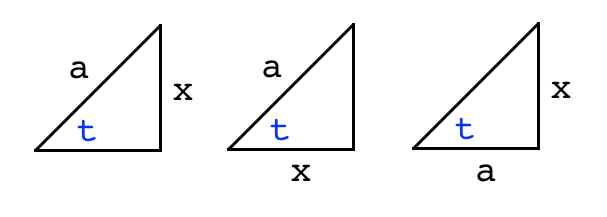
\includegraphics [scale=0.5] {trigints.png} \end{center}
In order from left to right, they are
\[ x = a \sin t, \ \ \ \ \sqrt{a^2-x^2} = a \cos t \]
\[ x = a \sec t, \ \ \ \ \sqrt{x^2-a^2} = a \tan t \]
\[ x = a \tan t, \ \ \ \ \sqrt{a^2+x^2} = a \sec t \]
It's common to see problems where $a$ is just $1$.  For example, suppose we integrate to find the area of a slice of the unit circle.  That is
\[ A = \int \sqrt{1-x^2} \ dx \]
To solve this, set 
\[ x = \sin t \]
\[ dx = \cos t \ dt \]
\[ \sqrt{1-x^2} = \cos t \]
\[ \int \sqrt{1-x^2} \ dx = \int \cos^2 t \ dt \]
We can work this integral using integration by parts (see the separate write-up on that).  Let
\[ u = \cos t \]
\[ dv = \cos t \ dt \]
Then
\[ du = - \sin t \ dt \]
\[ v = \sin t \]
The IBP formula is:
\[ \int u \ dv = uv - \int v \ du \]
\[ = \sin t \cos t + \int \sin^2 t \ dt \]
\[ = \sin t \cos t + \int 1 - \cos^2 t \ dt \]
\[ = \sin t \cos t + t - \int \cos^2 t \ dt \]
Thus
\[ 2 \int \cos^2 t \ dt = \sin t \cos t + t \]

Moving back to our problem, then
\[ \int \cos^2 t \ dt = \frac{1}{2}(t + \sin t \cos t) \]
\[ = \frac{1}{2}(\sin^{-1}x + x \sqrt{1-x^2}) \]
A diagram shows where these two terms come from
\begin{center} 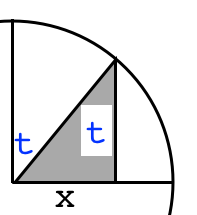
\includegraphics [scale=0.5] {area_int_trig.png} \end{center}
What is shown is a portion of the unit circle, and we're interested in the area under the graph between the limits $x=0 \rightarrow x=x_0$.  This area is broken up into two parts.  The height of the graph at $x$ is $\sqrt{1-x^2}$ so the area of the gray triangle is
\[ A = \frac{1}{2} x \ \sqrt{1-x^2} \]
The sine of the angle $t$ is $x$ (since the hypotenuse is equal to $1$) .  The angle $t$ is also the angle that sweeps out the sector of the circle as shown (because internal angles, etc.).  But this is just the ratio of $t$ to $2 \pi$ times the area of the (unit) circle
\[ A = \frac{t}{2 \pi} \pi r^2 = \frac{1}{2} t = \frac{1}{2} \sin^{-1} x \]
So the total area is
\[ A =  \frac{1}{2} (x\  \sqrt{1-x^2} + \sin^{-1} x) \]


A variation on the same problem yields a familiar result very quickly:
\[ \int \frac{1}{\sqrt{1-x^2}} \ dx = \frac{1}{\cos t} \cos t \ dt \]
\[ = \int dt = t \]
\[ \int \frac{1}{\sqrt{1-x^2}} \ dx = \sin^{-1} x \]

\end{document}  